花崗岩コアを伝播する弾性波を計測するため行った実験の方法について述べる。
以下でははじめに、実験に用いたコアサンプルについて、次に、強い弾性波を励起する
ために設計、制作した圧電超音波トランスデューサについて述べた後,計測システム全体の構成
と計測点の配置を示す。
\subsection{実験供試体}
超音波計測に用いた花崗岩供試体の外観と、形状および大きさを図\ref{fig:fig1}に示す。
供試体は、岡山県万成の採石場で採取した万成花崗岩を円柱状に加工したもので、直径は
約66mm, 高さは60mmである。主要造岩鉱物は石英、雲母、ナトリウムおよびカリ長石で。
数mmから数cm程度の結晶粒から構成される。外観からは肉眼で観察できるき裂などはなく、
風化もや造岩鉱物の明らかな変質も認められない。
ここで、供試体内部と表面の位置を指定するための$XYZ$直交座標を図\ref{fig:fig1}の
(b)および(c)のように取る。超音波の送信と受信は、供試体の上面$(Z=0)mm$で行い,
主として直径方向に伝播する表面波を観測する。
%--------------------
\begin{figure}[h]
	\begin{center}
	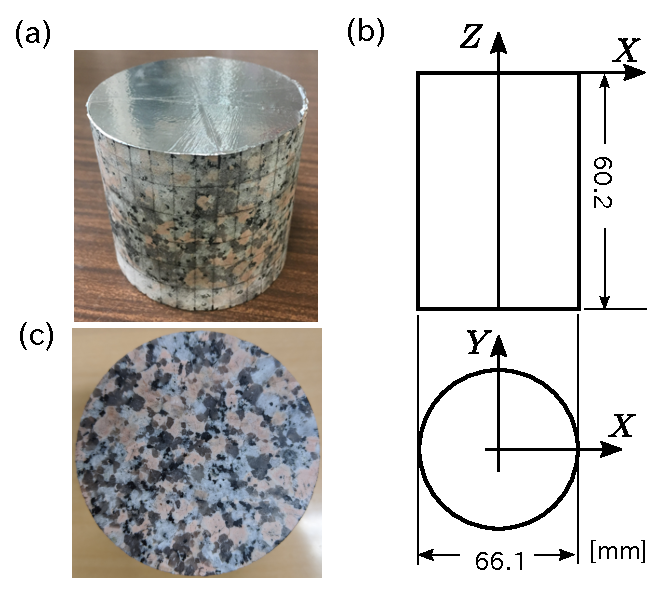
\includegraphics[width=0.6\linewidth]{Figs/fig1.eps} 
	\end{center}
	\caption{
		超音波計測に用いた花崗岩コア供試体(万成花崗岩).
	} 
	\label{fig:fig1}
\end{figure}
%--------------------
\subsection{超音波トランスデューサ}
本年度の実験のために、超音波を送信するための接触型ラインフォーカス・トランスデューサを設計、制作した。
圧電超音波トランスデューサの構成を図\ref{fig:fig2}に示す。
曲率をもった圧電素子がくさび状のポリエーテルイミドのシューにマウントされている。
圧電素子の曲率中心はシューの先端部にある。
シュー先端部の幅は1mmで、圧電素子の周波数は2MHz.
花崗岩試料の弾性波速度は、縦波が約5km/s, 横波が3km/s程度であることがわかっている。
そのため、2MHzの超音波の岩石試料内部での波長は縦波。横波のそれぞれ、およそ2.5mm, 1.5mm程度となる。
試料表面の方向に十分な強度の超音波を送信するためには、シュー先端の幅は波長程度の寸法にする必要がある。
ここでは、先端部の幅を2MHzの横波波長よりも小さくなるよう、1mmとした。
圧電素子の幅は、シュー先端部の幅と岩石中での超音波の波長よりも十分に長くなるよう
40mmとした。これにより、線音源に近い状態を作り、平面波を励起する。
完全な平面波は距離による減衰が無く、伝播挙動を理解しやすい。
このことは、岩石のような強い散乱減衰を起こす、不均質材中の弾性波挙動を調べる上で重要である。
%--------------------
\begin{figure}[h]
	\begin{center}
	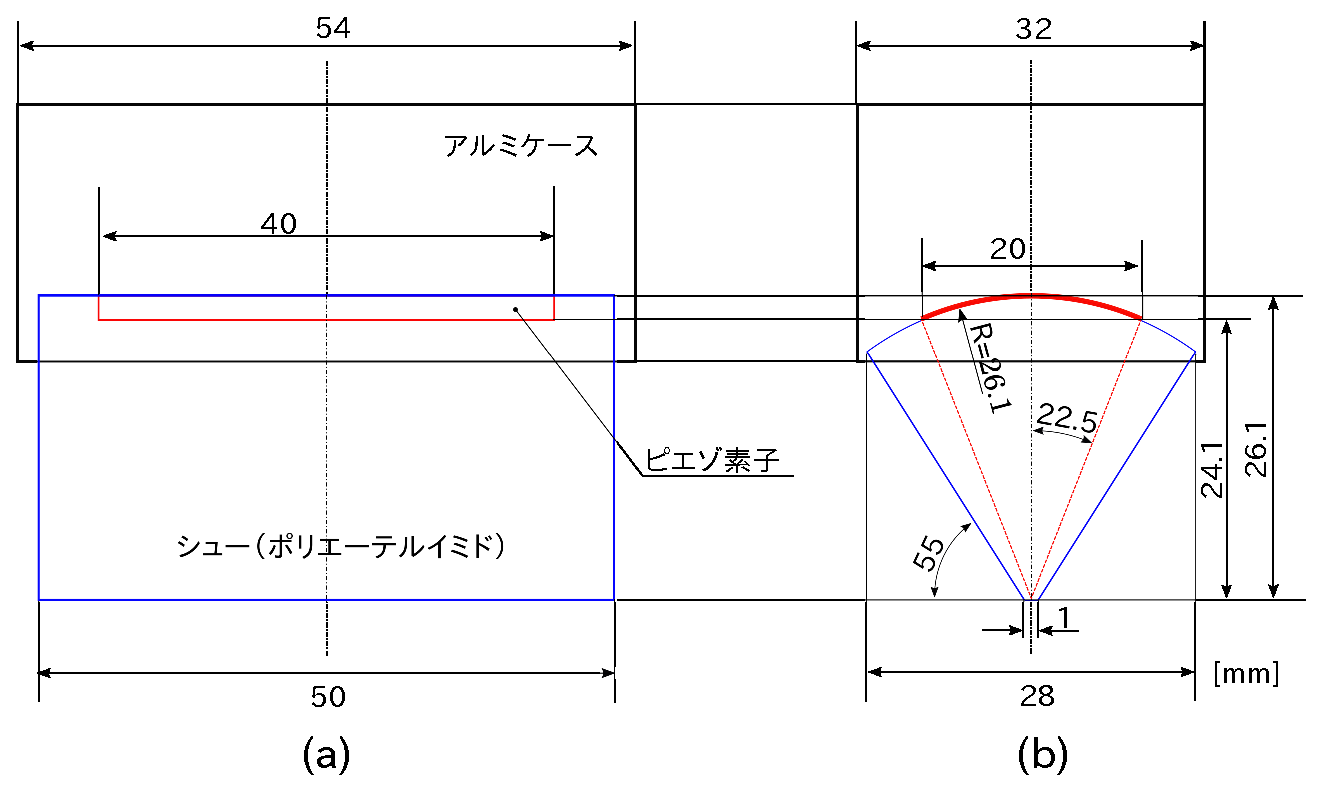
\includegraphics[width=0.8\linewidth]{Figs/fig2.eps} 
	\end{center}
	\caption{
		接触型ラインフォーカス探触子の形状と寸法.
	} 
	\label{fig:fig2}
\end{figure}
%--------------------
\subsection{超音波計測系の構成}
超音波計測システムの構成を図\ref{fig:fig3}に示す。
花崗岩コア試料は、3軸ステージ上に固定する。
3軸ステージは、平面内xy方向へ並進2軸、鉛直方向を回転軸とする回転1軸を持つ。
各ステージはステッピングモーターで駆動され、試料の位置と向きを正確に調整するために用いる。
送信に用いるラインフォーカストランスデューサは、コア供試体上面に接触させて固定する。
受信には、レーザードップラー振動計(LDV: laser Doppler vibrometer)を用いる。
LDVは、高い空間解像度と十分な周波数帯域を持つことから、ここでの計測に理想的なものである。
ただし、試料表面の状態により信号−雑音比(SN比)が大きく変化することが問題となる。
ここでは十分な反射レーザー光の受光感度を得るため、
コア供試体の上面にアルミ箔を貼り付けている。
アルミ箔は、供試体表面にオイルを均等に塗り、供試体とアルミ箔の間に空隙を残さないように貼り付けている。
送信に用いるトランスデューサは、超音波探傷試験用のパルサーレシーバから、矩形パルスを
印加して励起する。LDVは、LDVコントローラを介して制御PCとオシロスコープに接続する。
オシロスコープでは、LDVで計測した速度波形の取り込みを、パルサーレシーバと同期して行う。
一方、制御PCは、LDVコントローラ、オシロスコープとシリアル通信を行う。
PCとはLDVから受光感度のデータを受け取り、計測点毎にフォーカス調整機能を動作させる。
オシロスコープからはLDVから取り込みデジタイズされた波形を取得する。
また、制御PCは3軸ステージの移動をステージコントローラを介して行う。
以上、LDVのフォーカス調整、受光感度記録、波形取り込み,ステージ制御による計測点位置調整を、
本システムでは、PCからのシリアル通信によるコマンド制御で行うことで、一連の計測を自動化して行うことができる。
%--------------------
\begin{figure}[h]
	\begin{center}
	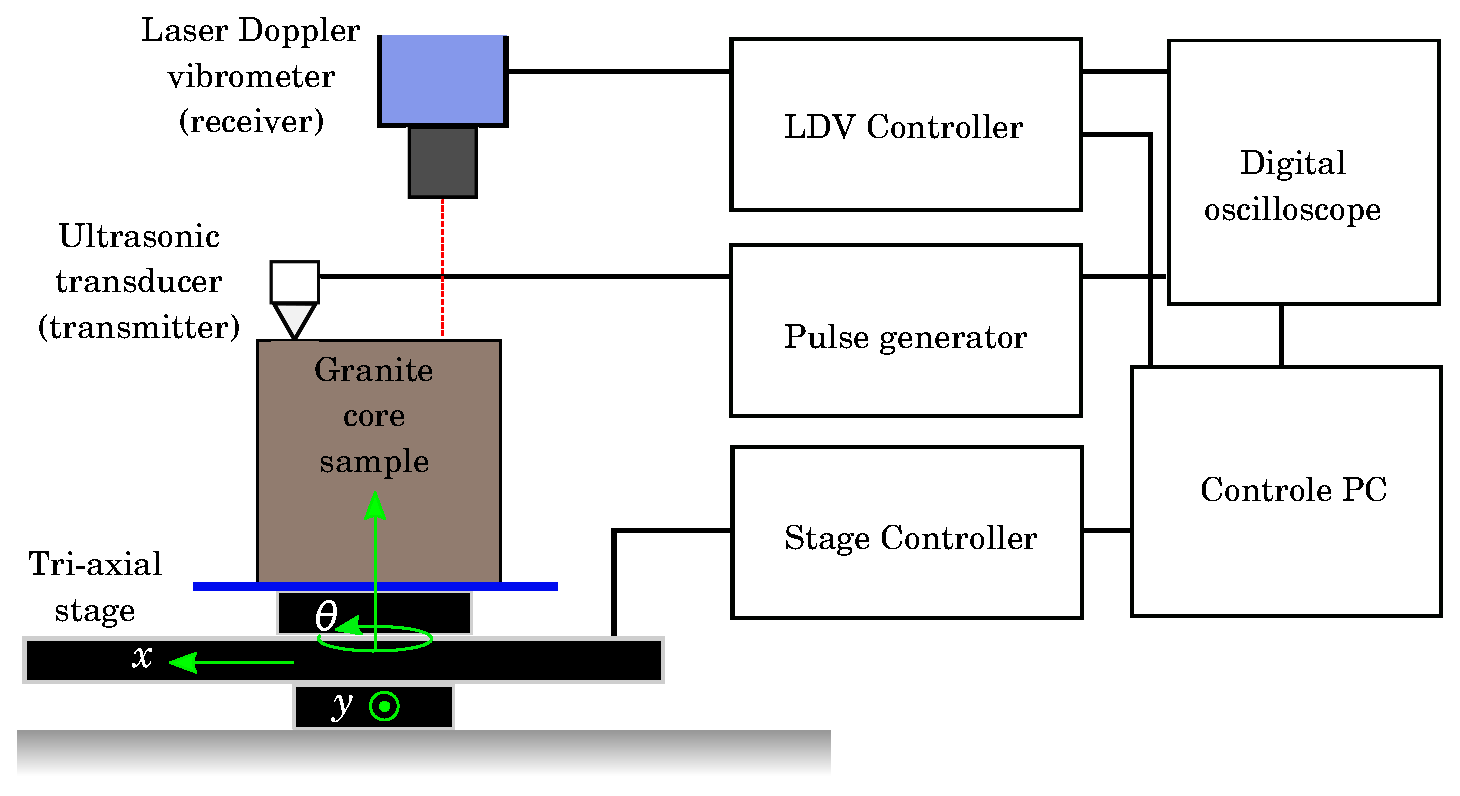
\includegraphics[width=0.8\linewidth]{Figs/fig3.eps} 
	\end{center}
	\caption{
		超音波測定装置の構成.
	} 
	\label{fig:fig3}
\end{figure}
%--------------------
\subsection{送受信点の配置}
超音波の送受信点位置を指定するために、図\ref{fig:fig4}に示すような
$xy$座標系を、供試体上面($Z=0$)にとる。$xy$座標は、$XY$座標と反時計回りの方向に
$\theta$だけ向きが異なるものとする。
ここで、$x$軸は、入射波の伝播方向を向くようにとることとする。
すなわち、X軸から測った角度$\theta$で入射波の伝播方向を表す。
$\theta$方向に超音波を入射するために、ラインフォーカストランスデューサは、
図\ref{fig:fig4}の$\cal S$で示した位置にシュー先端部を接触させて固定する。
一方、LDVによる超音波の受信は,同図で${\cal R}$として示した測線上を0.5mmのピッチで
行う。測線の長さは20mmとしているため、測定点数は41点となる。
送信位置$\cal S$、受信位置$\cal R$はは、いずれも
コア供試体の中心($(x,y)=(0,0)$mmから20mm離れた位置とし、これにより、40mmの距離
を伝播した超音波の上下動($Z$方向成分)を計測する。
このような計測を入射角$\theta$を0度から330度まで30度ピッチで行い、計12の入射
方向について供試体の直径方向に伝播する超音波の計測を行う。
\begin{enumerate}
\item パルサー設定
	\begin{itemize}
		\item 電圧パルス形状:矩形
		\item 印加電圧: -400V
		\item パルス幅: 0.25$\mu$sec 
		\item パルス繰り返し周波数:2kHz
	\end{itemize}
\item 波形収録条件
	\begin{itemize}
		\item サンプリング周波数:40MHz
		\item サンプリング点数:4,000点
		\item 計測時間範囲:0$\sim$100$\mu$sec
		\item 平均化回数:4,096回
	\end{itemize}
\item 送受信点配置
	\begin{itemize}
		\item 入射方向$\theta$[deg]:
			\[
				\left\{ 
				\theta=k \Delta \theta \left| \Delta \theta=30,\, k=0,1,\dots 11\right.
				\right\}
			\]
		\item 送信位置[mm]:
			\[
				{\cal S}=\left\{ (x,y)\left| x=-20, |y| \leq 20\right.\right\}, \ \ 
			\]
		\item 受信位置[mm]:
			\[
				{\cal R}=\left\{ (x,y)\left| x=20,  |y| \leq 10\right.\right\}, \ \ 
			\](0.5mmピッチ)
		\item 透過距離:$L$=40mm
	\end{itemize}
\end{enumerate}
%--------------------
\begin{figure}[h]
	\begin{center}
	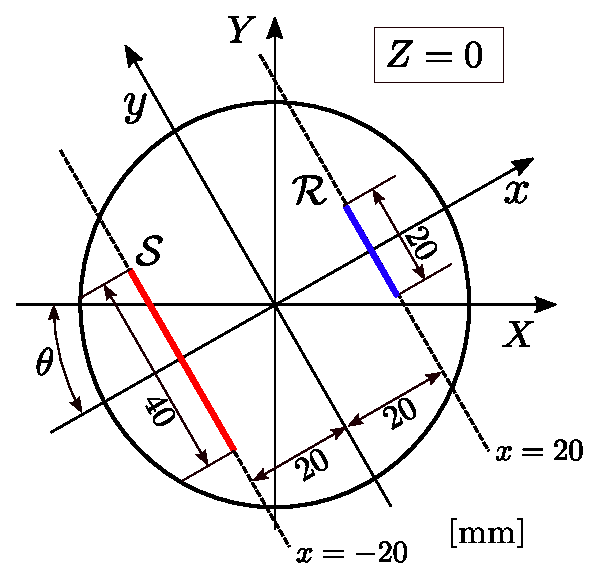
\includegraphics[width=0.5\linewidth]{Figs/fig4.eps} 
	\end{center}
	\caption{
		花崗岩コア供試体の上面における超音波送受信位置の配置.
		${\cal S}$は,ラインフォーカス探触子のカップリング位置を,
		${\cal R}$は,レーザー振動計による計測の測線を表す.
	} 
	\label{fig:fig4}
\end{figure}
%--------------------

